\section{Target gene analysis}

As discussed in \cref{sec:circrna_functions}, \glspl{crna} can act as
\gls{mirna} sponges and regulate the expression of target genes.
In order to investigate this regulatory mechanism, the \gls{nf-circrna}
pipeline was used to predict interactions between differentially expressed
\glspl{crna} and \glspl{mirna} that are known to be active in mouse mammary
tissue.
The dataset introduced in \cref{sec:mirna_data} was used for this analysis.
It provides a list of identified \glspl{mirna} and the target genes they are
predicted to regulate.

For each of the differentially expressed \glspl{crna}, the pipeline predicted
potential interactions with \glspl{mirna} based on sequence complementarity and
binding energy calculations.
For each \gls{crna}, the target genes of all \glspl{mirna} it interacts with
were aggregated to a single list of potential \gls{crna} target genes.
Then, gene set enrichment analysis was performed using ClusterProfiler to
identify biological processes and pathways that are significantly enriched
among the predicted target genes.

When analyzing the results, it is important to consider that the predictions
are based on the entire sequence of the \gls{crna} between the \gls{bsj} sites.
Thus, regions of the \gls{crna} that are not part of the \gls{fli} are also
considered in the analysis, which may lead to false positive predictions.

The results of the target gene analysis for the differentially expressed
\glspl{crna} are shown in \cref{fig:target_genes}.

\begin{figure}[H] \begin{tabular}{ccc} \begin{subfigure}{0.5\textwidth}
                  \centering

                  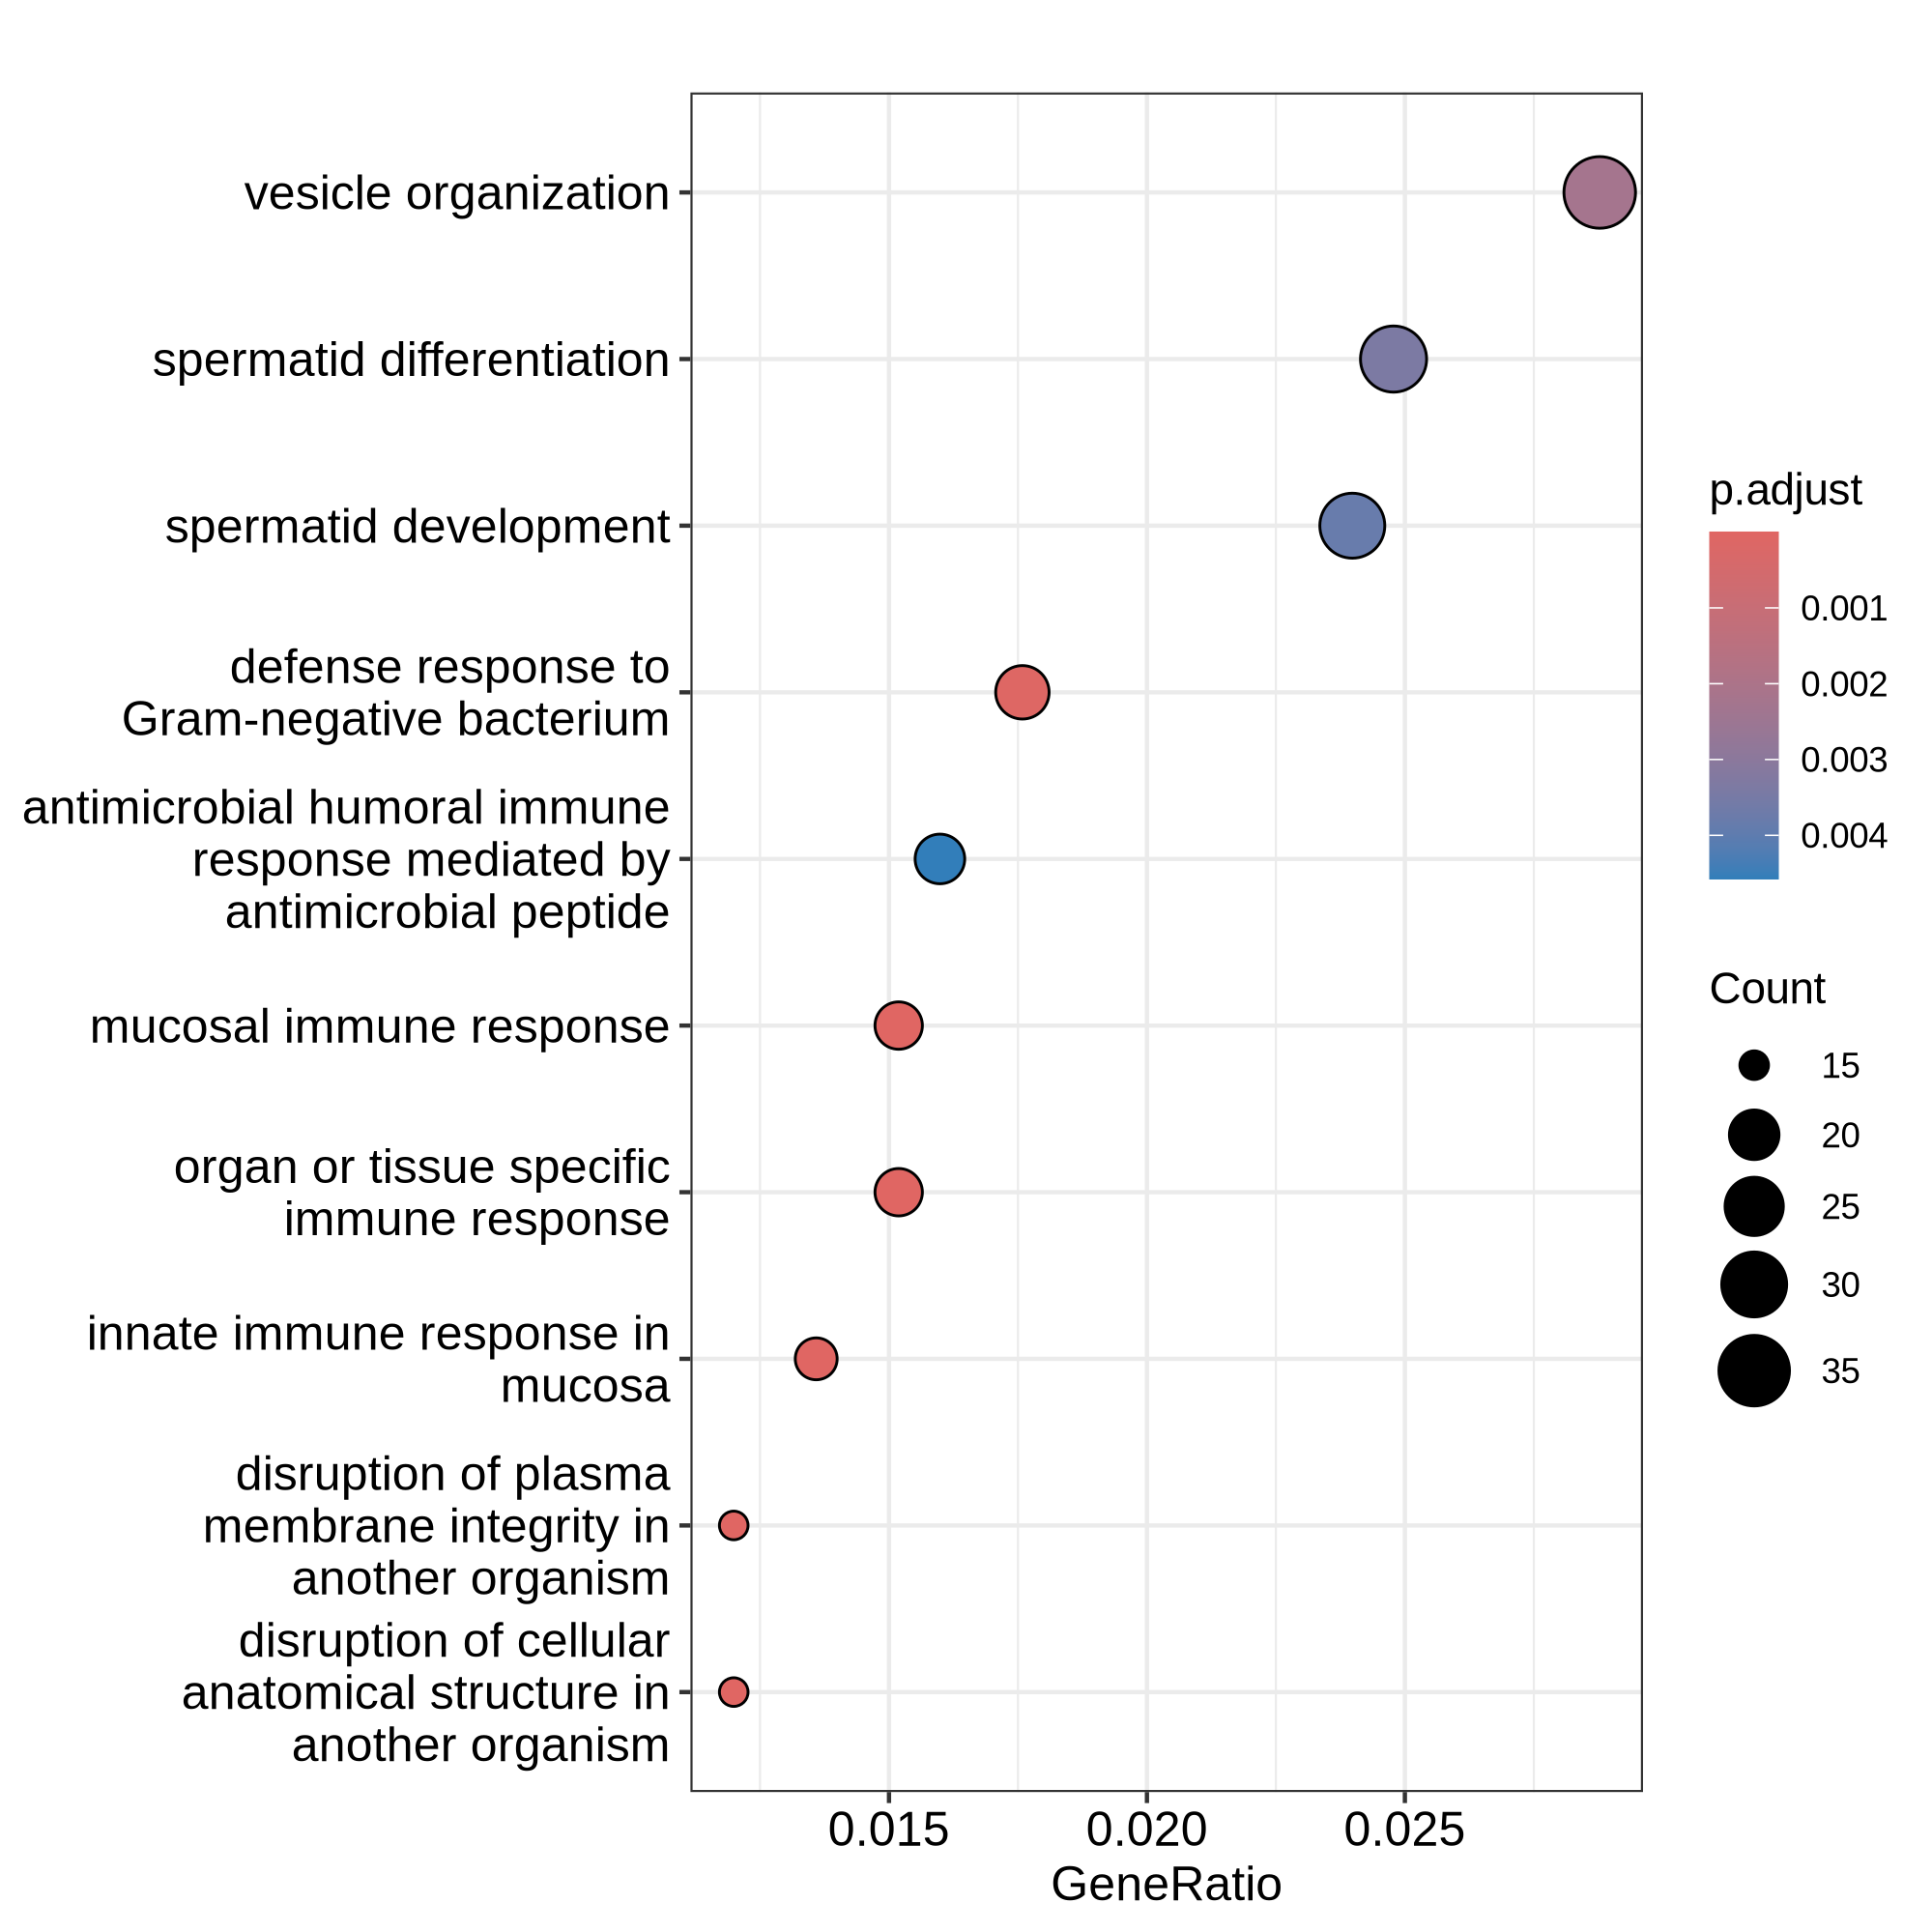
\includegraphics[width=\linewidth]{chapters/4_results_and_discussion/figures/dea/deseq2/letrozole/chr5:87925915-87926842_targets.txt.png}
                  \caption{Top 10 enriched \gls{go} terms in the target
                      genes of the \textit{Csn1s2a} \gls{crna}.
                  }
                  \label{fig:tg_csn1s2a}
              \end{subfigure}
        \begin{subfigure}{0.5\textwidth}
            \centering

            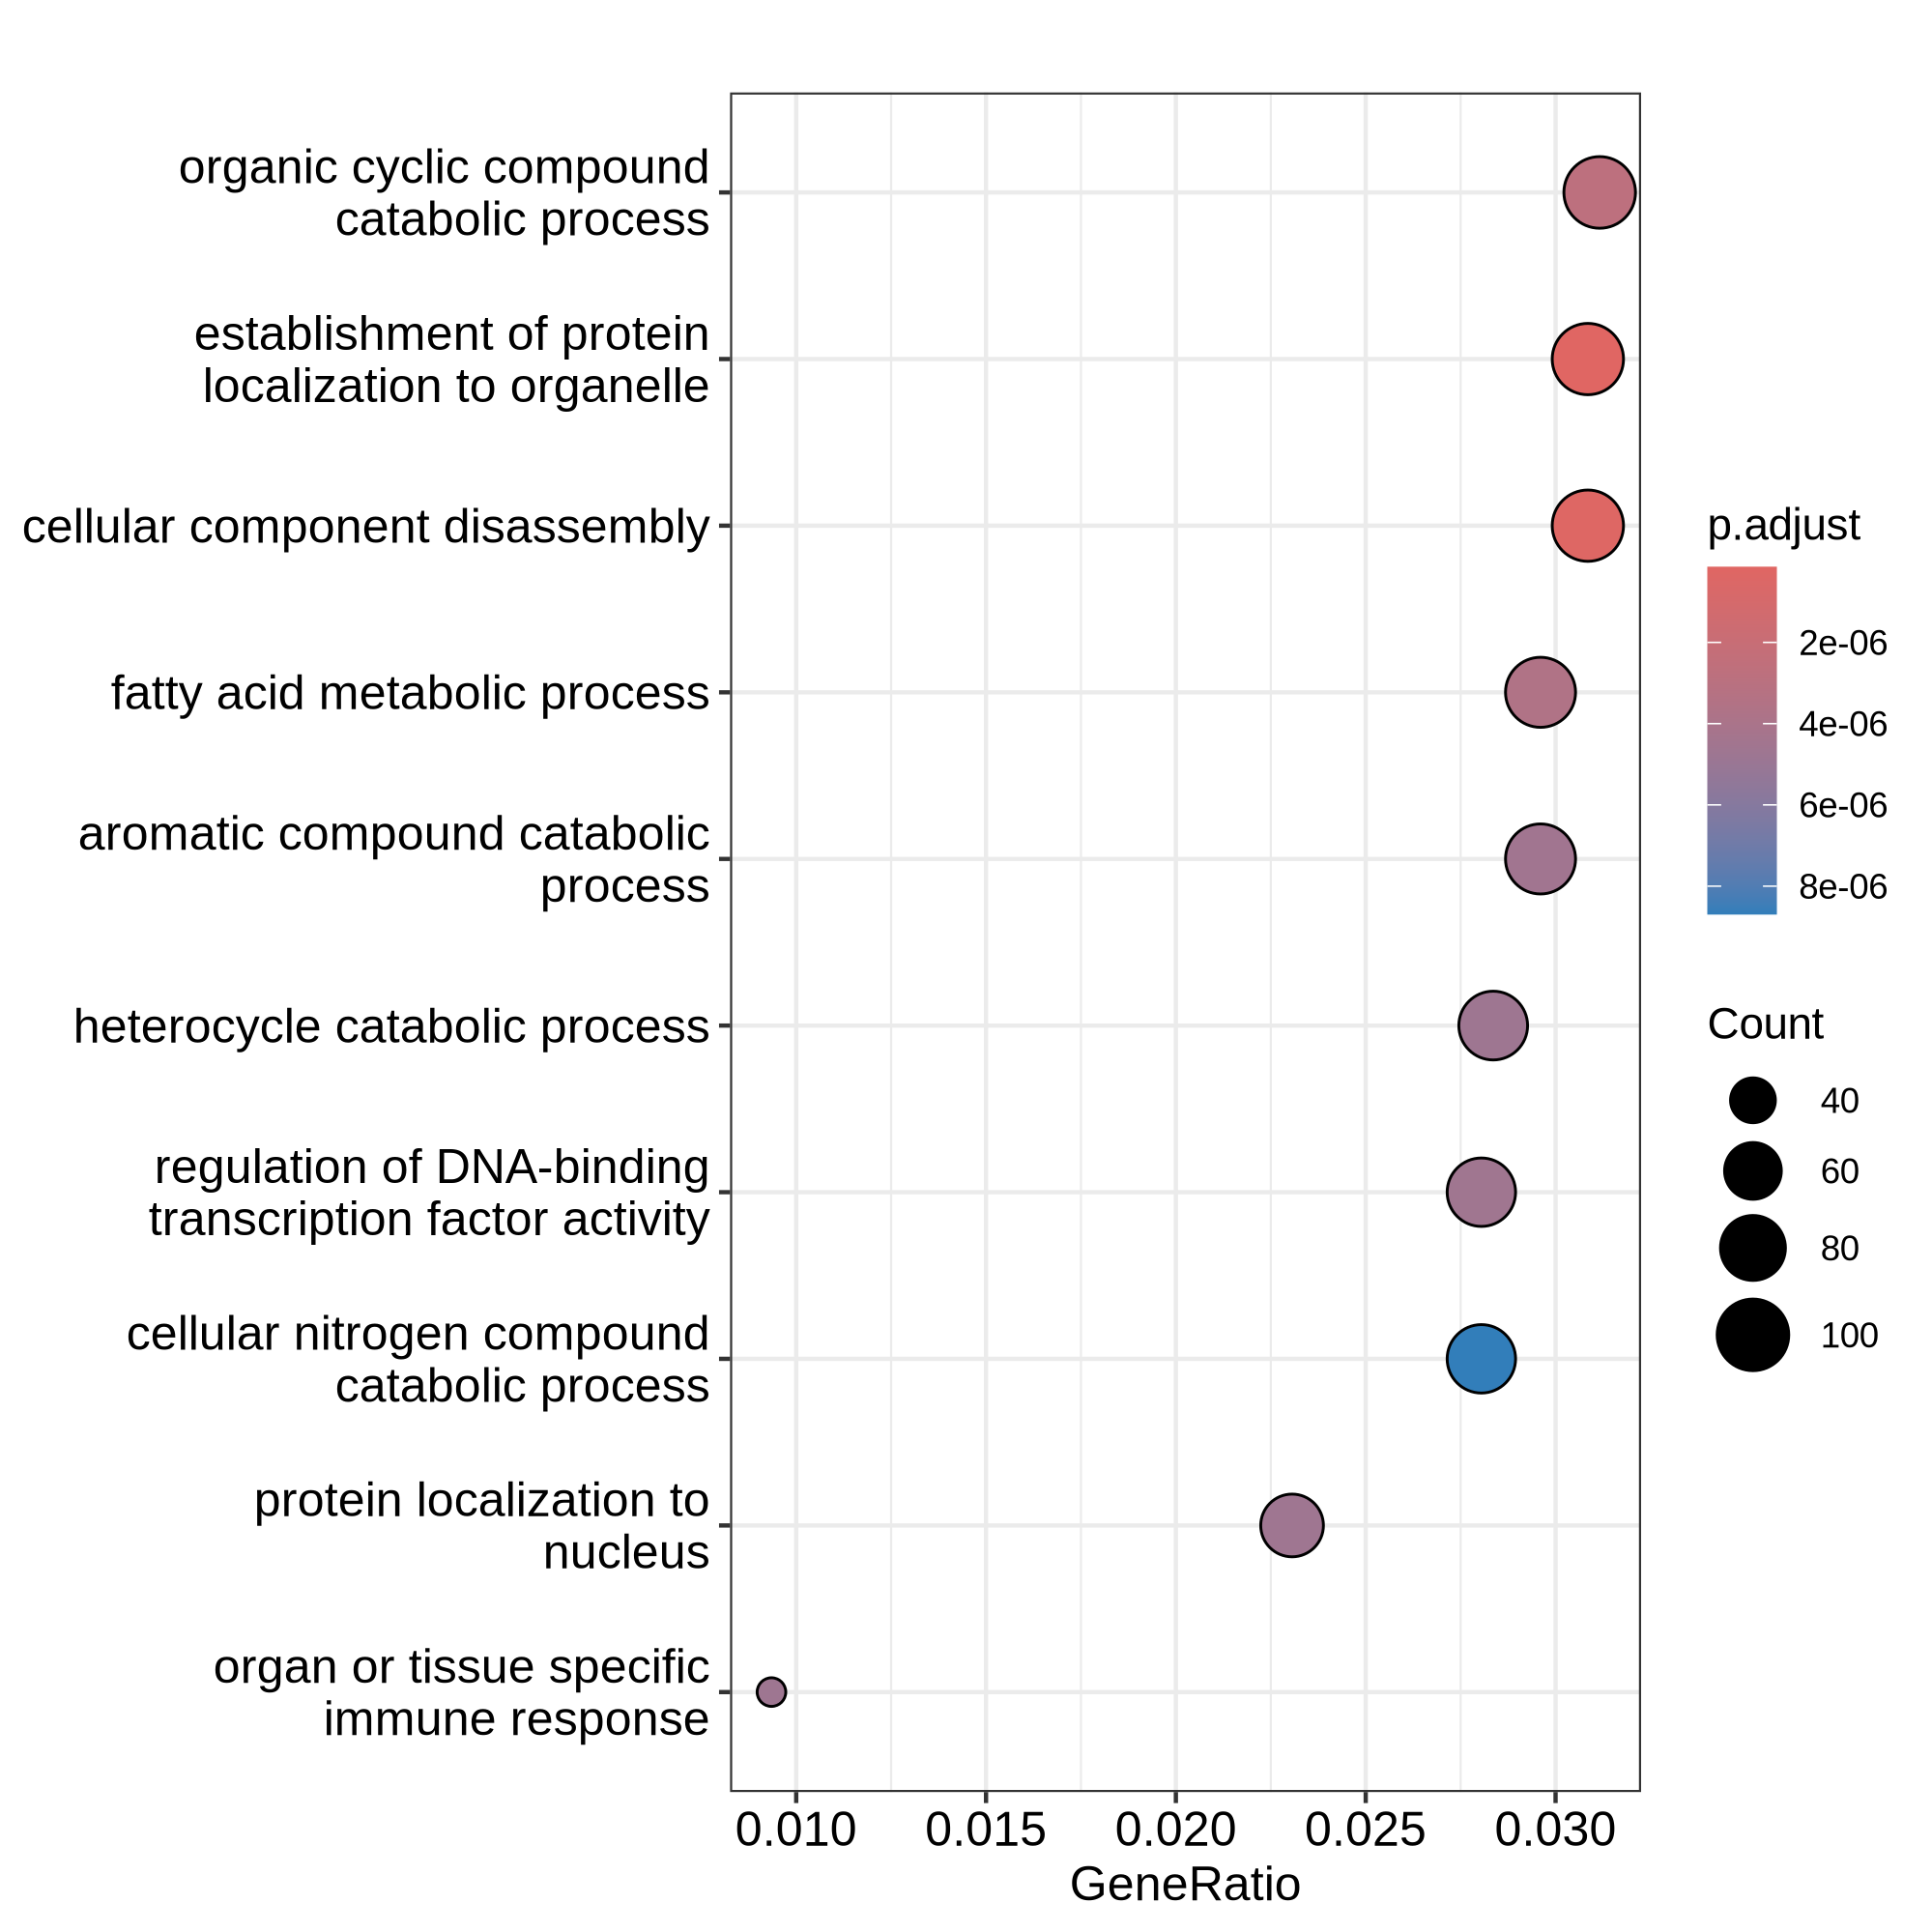
\includegraphics[width=\linewidth]{chapters/4_results_and_discussion/figures/dea/deseq2/letrozole/chr5:87817372-87821139_targets.txt.png}
            \caption{Top 10 enriched \gls{go} terms in the target
                genes of the \textit{Csn1s1} \gls{crna}.
            }
            \label{fig:tg_csn1s1}
        \end{subfigure}
    \end{tabular}
    \caption{Dot plots showing the top 10 enriched terms in the target genes of
        the \textit{Csn1s2a} and \textit{Csn1s1} \glspl{crna}.
        The \textit{Bbs9} \gls{crna} is not shown here, as no \gls{mirna} targets were
        predicted for this \gls{crna}.
    }
    \label{fig:target_genes}
\end{figure}

While the \textit{Bbs9} \gls{crna} did not have any predicted \gls{mirna}
targets, the target genes of the \textit{Csn1s2a} and \textit{Csn1s1}
\glspl{crna} showed significant enrichment in several biological processes and
pathways.

\subsection{Target genes of the \textit{Csn1s2a} \gls{crna}}

\subsection{Target genes of the \textit{Csn1s1} \gls{crna}}

